\chapter{Manuel}

\section{Manuel d'installation}
% Par : Fabien
% Relu : Florian, Clément, Oualid, Thin

Concernant l'hébergement du site chez un hébergeur web (Hostinger par exemple car il possède une version récente de PHP ainsi que tous les outils nécessaires à la mise en place du projet avec Symfony2) vous devez lui transmettre via FTP (par exemple FileZilla (voir \cite{fz})) l'ensemble des fichiers en conservant la structure actuelle des dossiers, à savoir :
\begin{itemize}
    \item app~;
    \item bin~;
    \item public\_html (et non web)~;
    \item src~;
    \item vendor~;
\end{itemize}
Ainsi que les différents fichiers situés à la racine du projet.

En cas de page blanche lors de l'accès au site en ligne vous devez vérifier qu'il n'y ait pas d'erreurs dans le code du projet car ceci arrive régulièrement et aucune erreur n'est décelée (la correction de ces problèmes peut se faire en local ou en distant via app\_dev.php et non app.php car l'erreur apparaît clairement par ce biais et devient facilement solvable).

Aussi, pour vérifier que tout fonctionne chez l'hébergeur vous devez pouvoir accéder au fichier \verb|config.php| situé à la racine de votre site et il ne doit y avoir aucune erreur sur cette page, si tel n'est pas le cas alors vérifiez le fichier \verb|config.php| du dossier public\_html. Si vous ne disposez pas des droits d'accès aux fichiers vous devez ajouter votre adresse ip, dans \verb|app_dev.php| à la ligne 
\verb|!in_array| \verb|(@$_SERVER['REMOTE_ADDR'],| \verb|array('127.0.0.1',| \verb|'fe80::1',| \verb|'::1'))| et dans \verb|config.php| aux lignes~:
\begin{lstlisting}
if (!in_array(@$_SERVER['REMOTE_ADDR'], array(
    '127.0.0.1',
    '::1',
))) {
    header('HTTP/1.0 403 Forbidden');
    exit('This script is only accessible from localhost.');
}
\end{lstlisting}

Ainsi, vous disposerez de votre site en production.
Encore une chose, il faut faire attention car chez certains hébergeurs le Système de Gestion de Bases de Données (SGBD) respecte la casse, dans ce cas, vous devrez modifier à la main le nom des tables dans ce même SGBD en les mettant sous la forme «~UpperCamelCase~» autrement les tables ne seront pas reconnues lors de l'exécution des requêtes utilisées dans le programme.

\section{Manuel d'utilisation}
% Par : Fabien
% Relu : Florian, Clément

Un visiteur peut accéder aux différentes informations sur le Système d'Echange Local, la monnaie libre. Il peut aussi s'inscrire par le biais de son prénom, de son nom, d'un login ainsi que d'un mot de passe. Avec ces deux derniers il peut se connecter (voir figure \ref{fig:Inscription}).

\begin{figure}[h!]
\centering
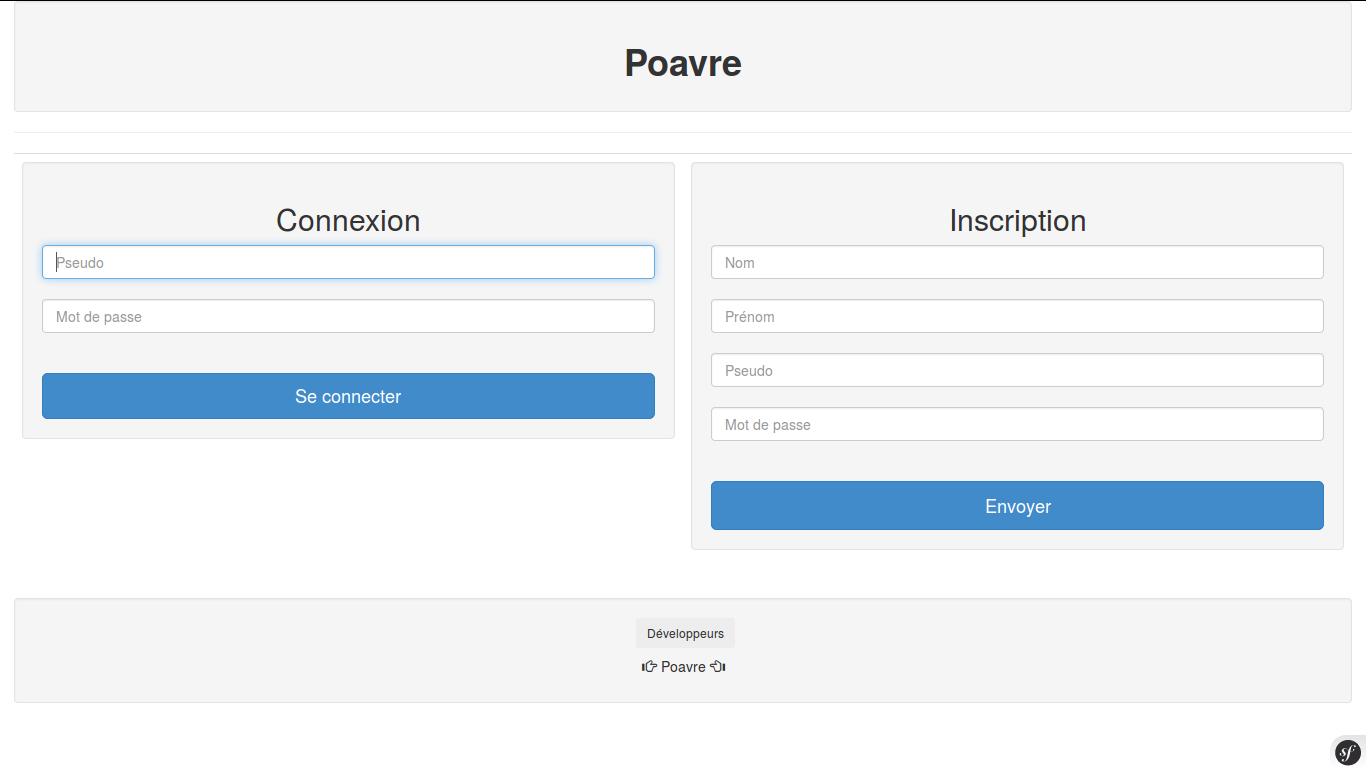
\includegraphics[width=0.9\textwidth]{inscription}
\caption{Capture d'écran d'une inscription/connexion}
\label{fig:Inscription}
\end{figure}

Lorsque le visiteur désormais nommé utilisateur est connecté (voir figure \ref{fig:Profil}) il peut à tout moment se déconnecter, éditer son profil (nom, prénom et/ou mot de passe).

\begin{figure}[h!]
\centering
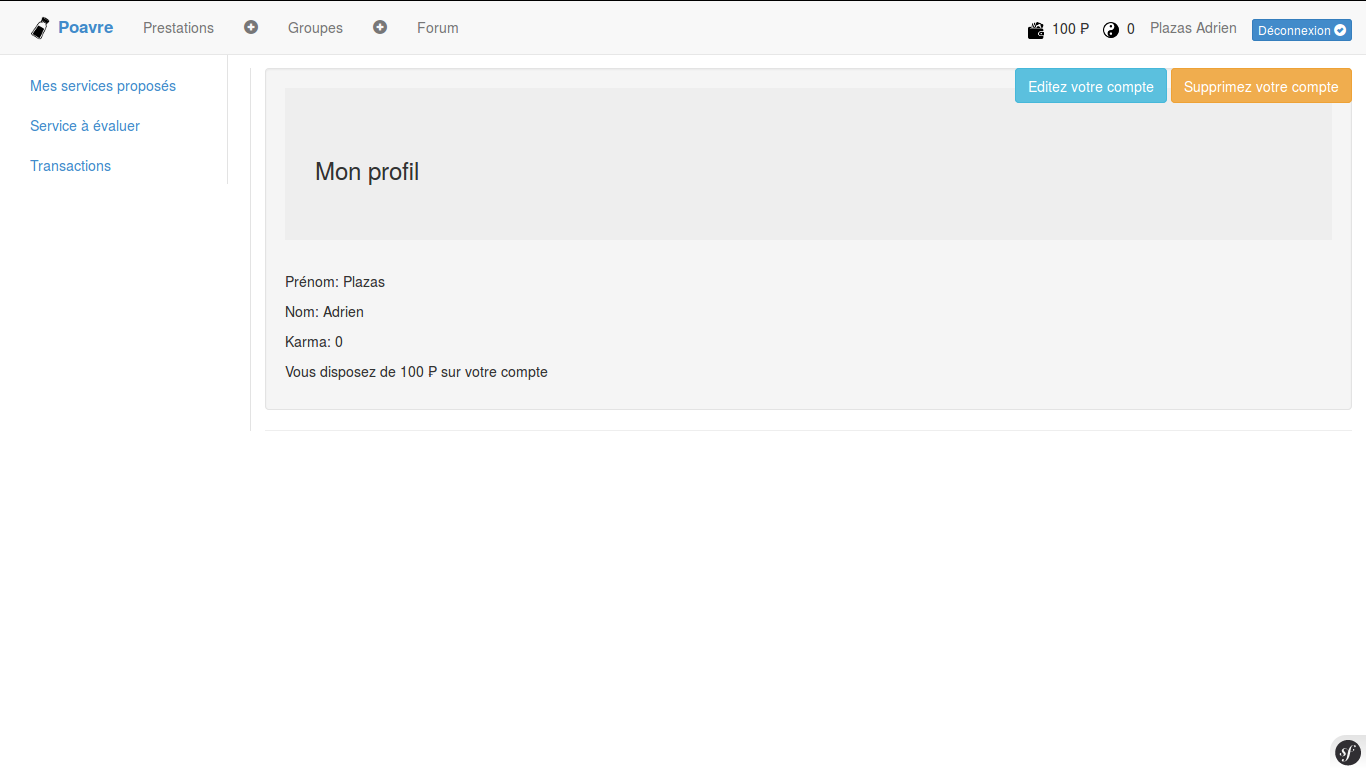
\includegraphics[width=0.9\textwidth]{profil}
\caption{Capture d'écran du profil}
\label{fig:Profil}
\end{figure}

Il peut accéder aux différents services proposés sur le site. 
Ces derniers peuvent être des services de covoiturage, de couchsurfing, de vente ou un autre type de service nommé «~service de base~».

Ainsi, il peut réserver un service, dans ce cas, le créateur du service se doit de le réaliser ce qui entraînera par la suite une obligation de transaction entre l'utilisateur et le créateur du service ainsi qu'une évaluation par la personne ayant bénéficiée du service (voir figure \ref{fig:Montre}).

\begin{figure}[h!]
\centering
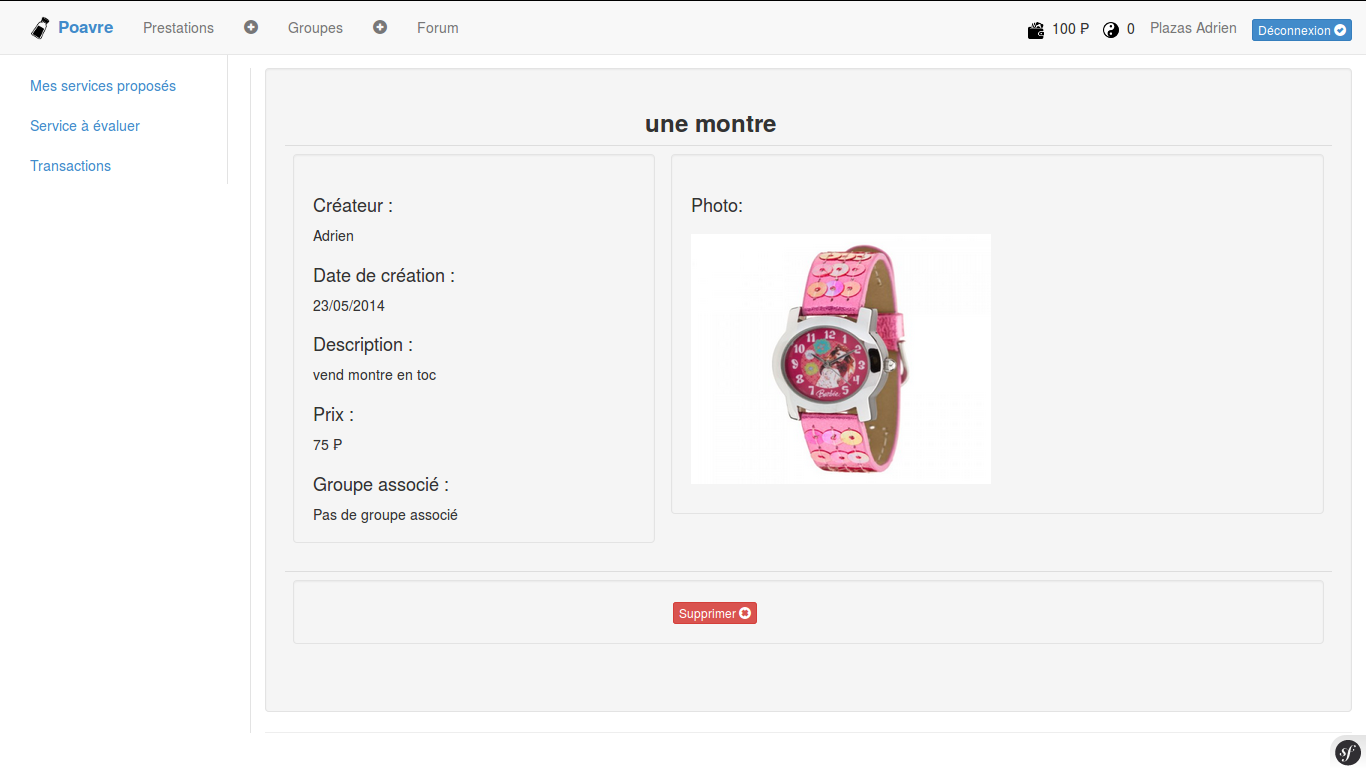
\includegraphics[width=0.9\textwidth]{montre}
\caption{Capture d'écran d'une réservation}
\label{fig:Montre}
\end{figure}

Chaque utilisateur peut également créer son propre service, il peut à tout moment l'annuler, il disparaît ainsi de la liste des services proposés sur le site (voir figure \ref{fig:Vente}).

\begin{figure}[h!]
\centering
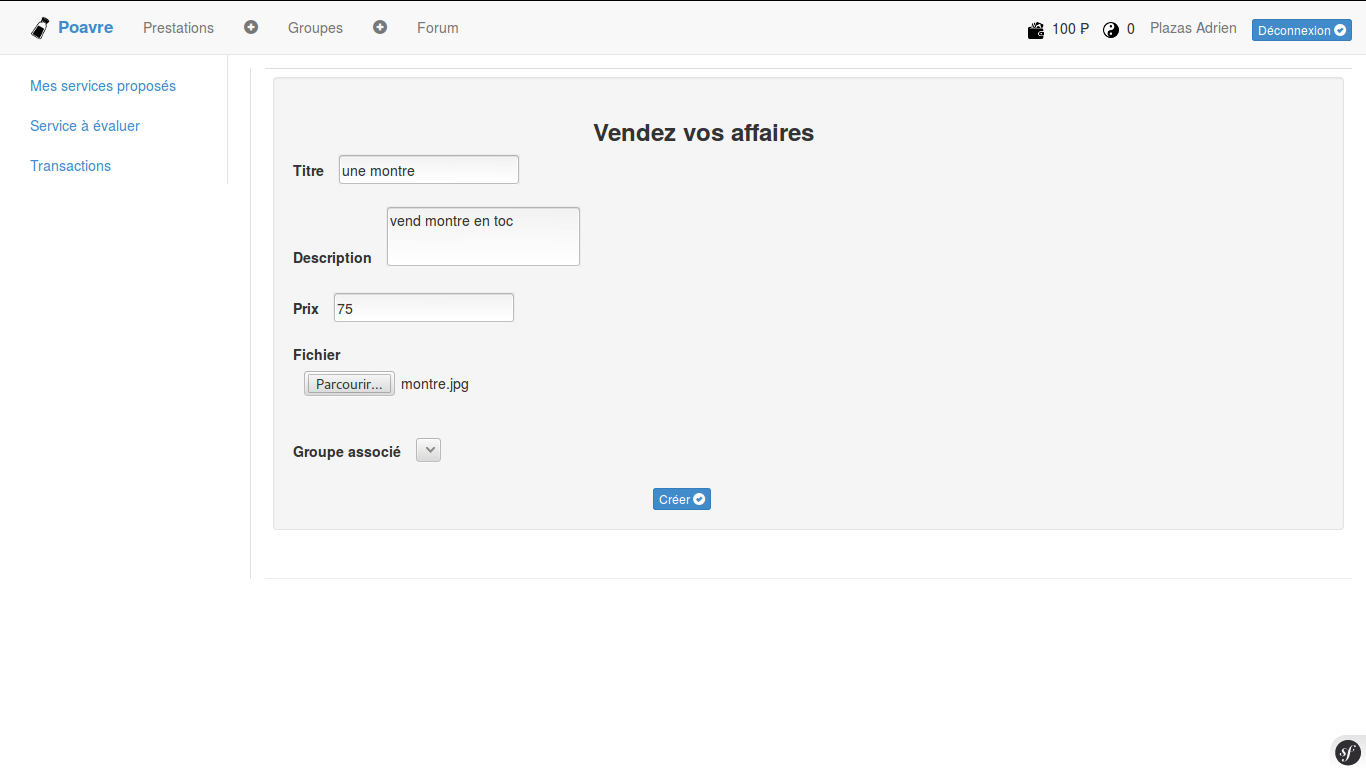
\includegraphics[width=0.9\textwidth]{vente}
\caption{Capture d'écran d'une vente}
\label{fig:Vente}
\end{figure}

L'utilisateur ne peut quitter le site que s'il a clôturé tous les services qu'il a réservé (un mail de contact est cependant disponible pour une suppression complète).
Par ailleurs, un utilisateur peut voir la liste des groupes présents sur le site, il peut candidater pour rejoindre ces différents groupes et peut à tout moment annuler sa demande. Il peut aussi visualiser pour chaque groupe la liste de ses membres ainsi que les services qui lui sont associés.
Lorsque l'utilisateur fait parti d'un groupe il peut quitter ce dernier s'il le souhaite.
Un utilisateur peut aussi créer son propre groupe en ajoutant des utilisateurs à ce dernier. Seuls un nom de groupe et une description sont demandés pour la création d'un groupe.
Un administrateur de groupe peut bannir les membres du groupe ou en ajouter de nouveaux et il peut voir la liste des candidatures pour rejoindre le groupe et les accepter ou refuser.
Il peut à tout moment dissoudre le groupe, dans ce cas, tous les services associés au groupe ne le sont plus, ils ne disparaissent cependant pas du site (voir figure \ref{fig:Groupe}).

\begin{figure}[h!]
\centering
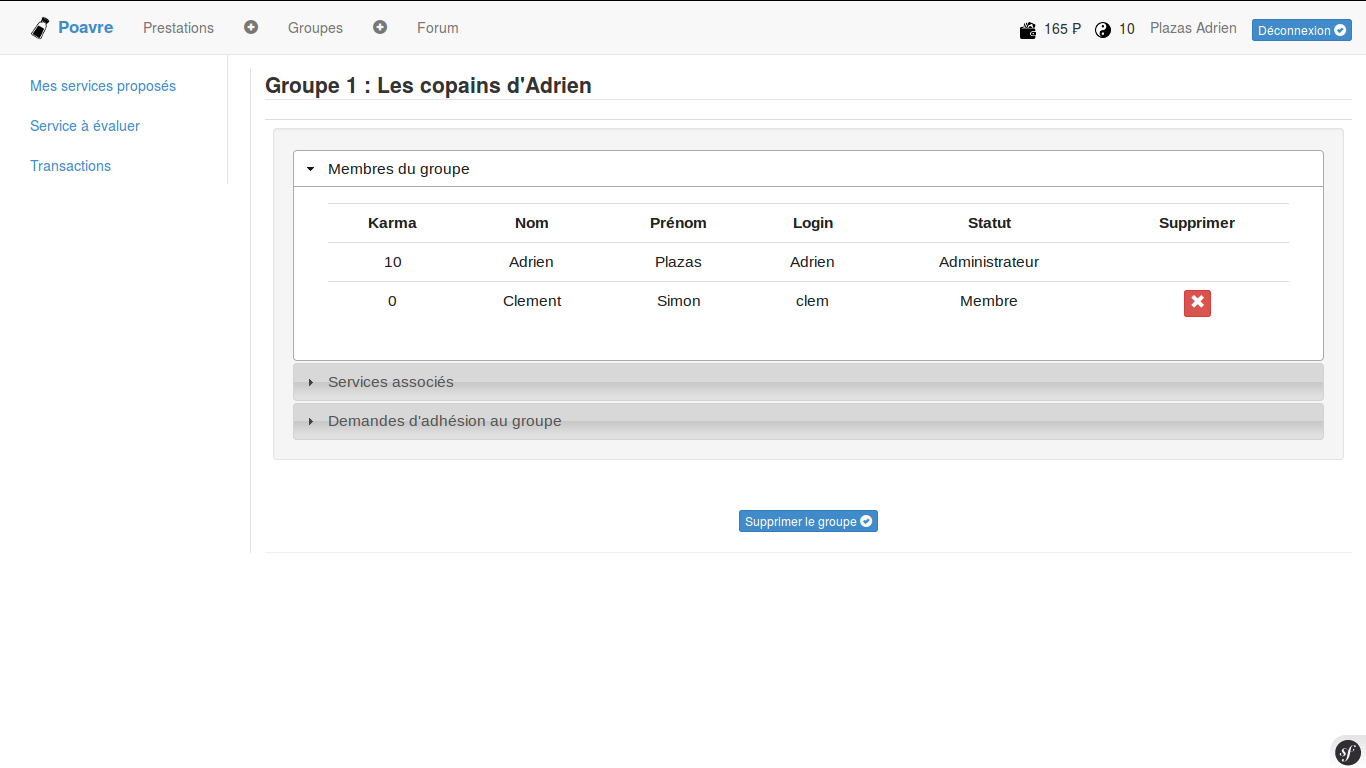
\includegraphics[width=0.9\textwidth]{groupe}
\caption{Capture d'écran d'un groupe}
\label{fig:Groupe}
\end{figure}

Un membre du site peut accéder aux différents services qu'il propose ainsi qu'aux services qu'on lui a réservé. Par ce dernier cas, il peut confirmer qu'un service a bien été effectué et après cela il peut évaluer le membre qui a réalisé le service. 
Cette évaluation permet à ce dernier d'obtenir des points de karma et déclenche la transaction entre les deux utilisateurs (voir figure \ref{fig:Evaluation}).

\begin{figure}[h!]
\centering
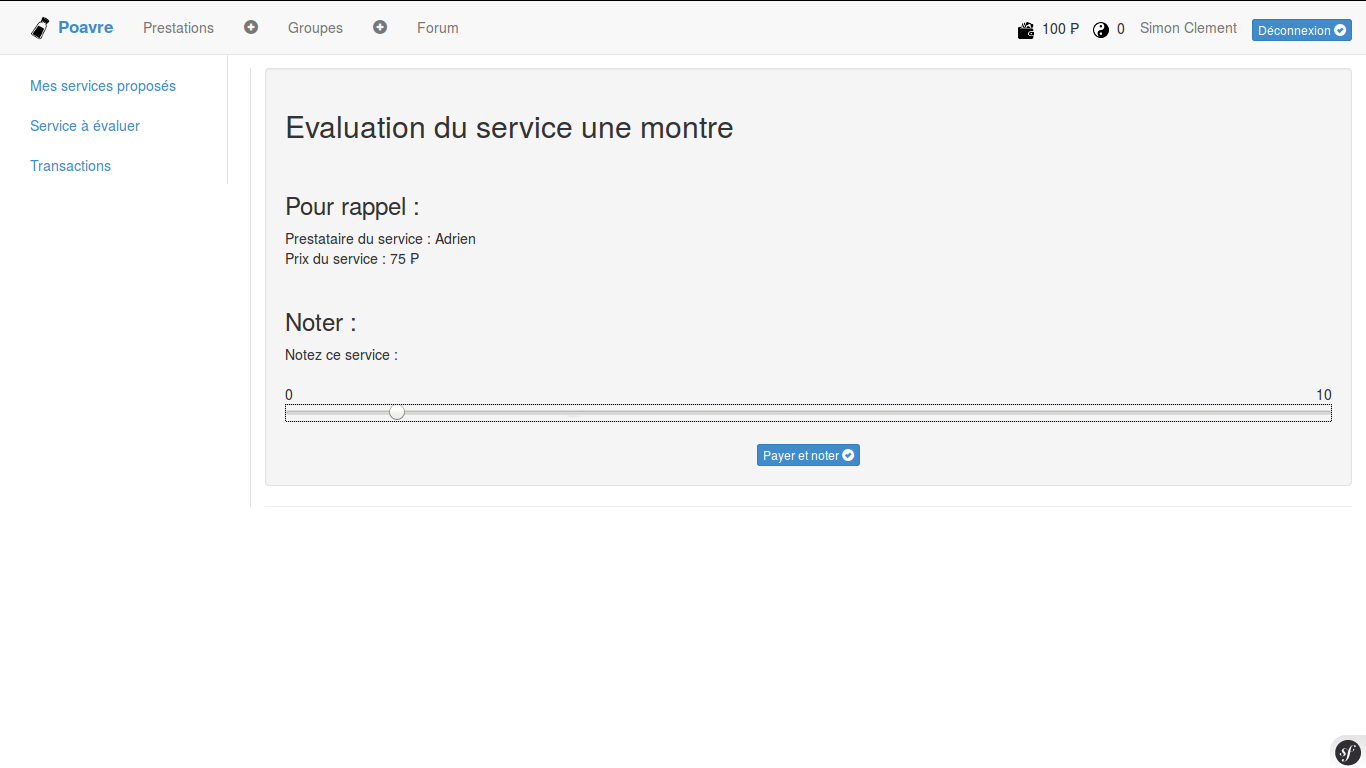
\includegraphics[width=0.9\textwidth]{achat}
\caption{Capture d'écran d'une évaluation}
\label{fig:Evaluation}
\end{figure}

A tout moment l'utilisateur peut visualiser le nombre de points de karma dont il dispose ainsi que l'argent qu'il possède.
Un utilisateur ne peut réserver un service que s'il dispose des fonds nécessaires pour payer le service (l'argent qu'il doit à un autre utilisateur est pris en compte dans ce calcul).
L'utilisateur peut visualiser la liste de ses transactions avec les autres utilisateurs et peut réaliser des paiements qualifiés de «~dons~» avec les autres utilisateurs (voir figure \ref{fig:Transaction}).

\begin{figure}[h!]
\centering
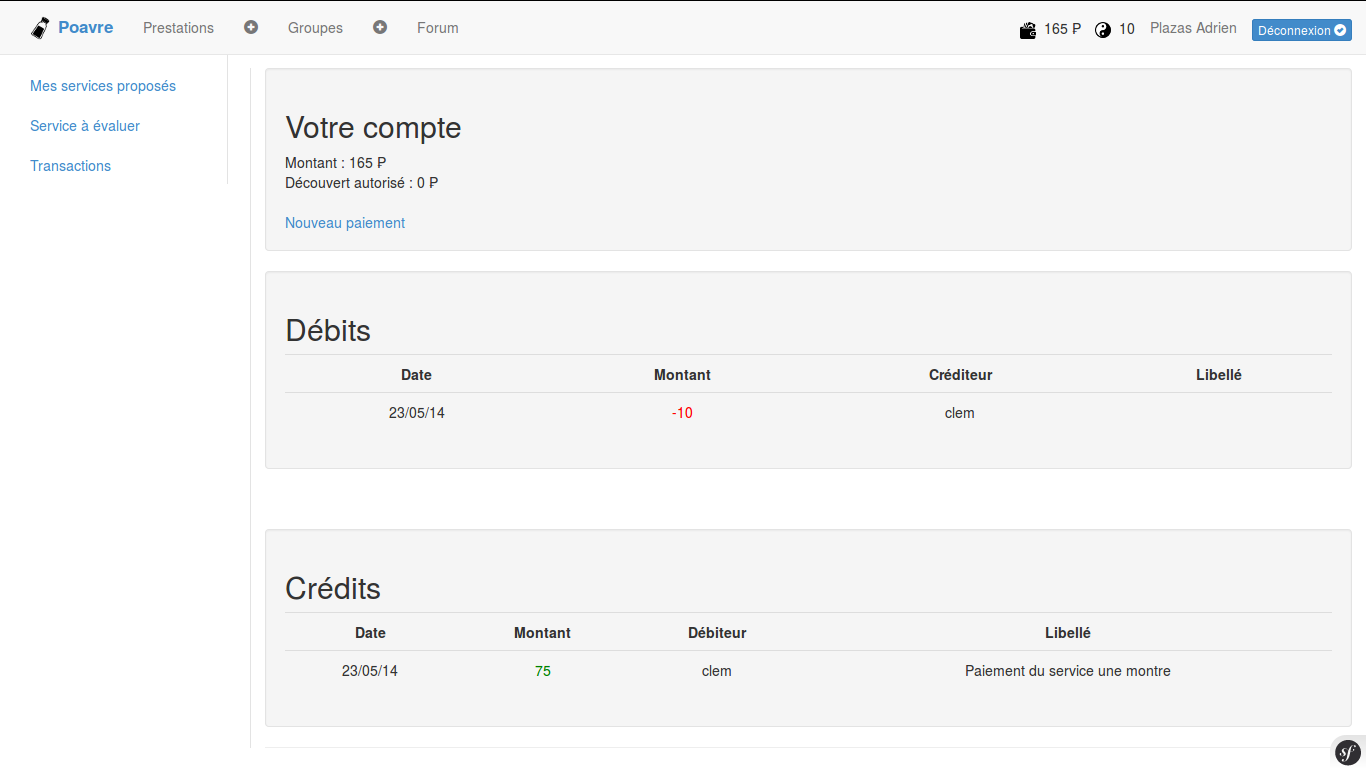
\includegraphics[width=0.9\textwidth]{trans}
\caption{Capture d'écran d'une transaction}
\label{fig:Transaction}
\end{figure}

Un membre du site peut accéder au Forum, par celui-ci il peut visualiser la liste des différents «~topics~» (ou «~sujets~») classés par ratios («~likes~»/«~dislikes~») décroissants (voir figure \ref{fig:Liste_Forum}).

\begin{figure}[h!]
\centering
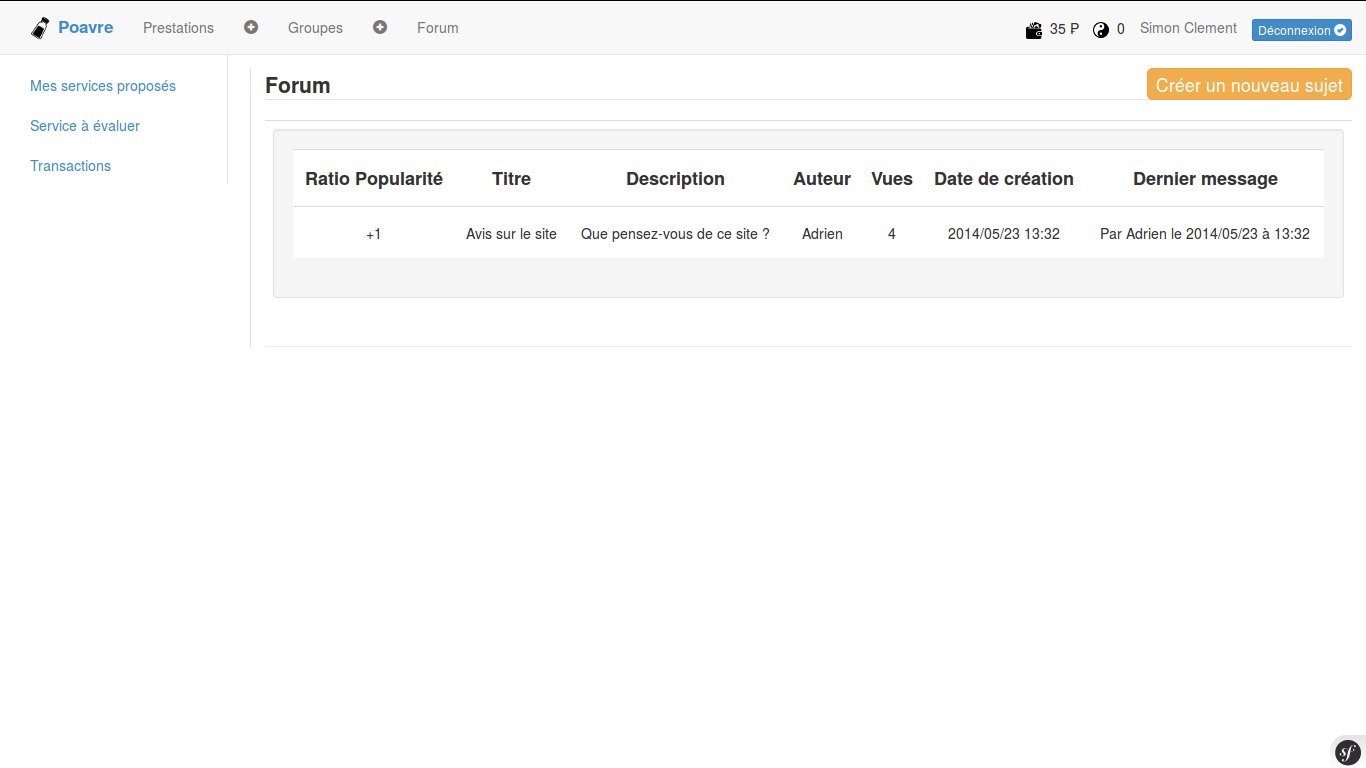
\includegraphics[width=0.9\textwidth]{liste_forum}
\caption{Capture d'écran de la liste des topics}
\label{fig:Liste_Forum}
\end{figure}

Il peut ainsi accéder à un topic, commenter celui-ci ou encore l'évaluer par un «~like~» ou un «~dislike~». 
Bien évidemment l'utilisateur peut lui-même créer un topic (voir figure \ref{fig:Forum}).

\begin{figure}[h!]
\centering
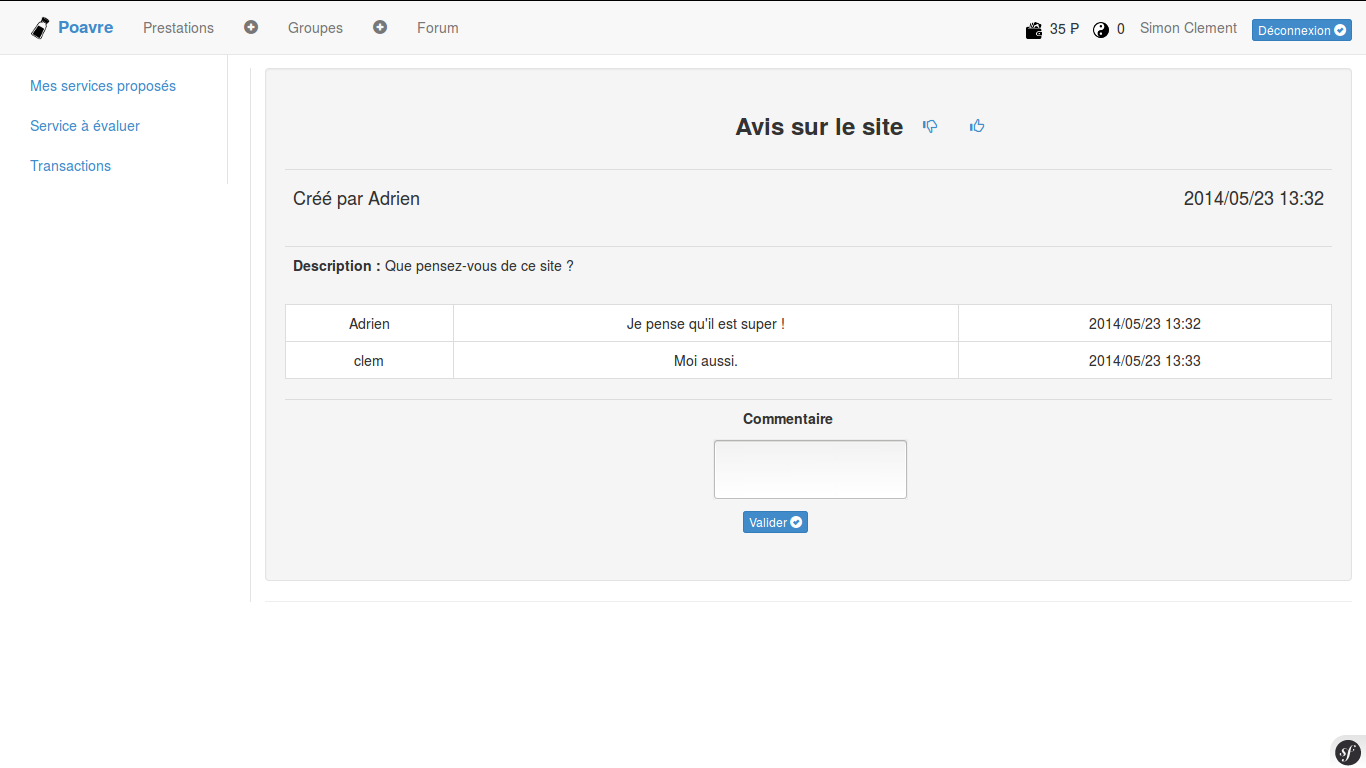
\includegraphics[width=0.9\textwidth]{forum}
\caption{Capture d'écran du forum}
\label{fig:Forum}
\end{figure}

De plus, un utilisateur bénéficiant des droits d'administration peut accéder à l'espace d'administration du site.
Depuis ce dernier, il peut bannir des utilisateurs, leur accorder les droits d'administration ou les droits «~suprêmes~», il peut aussi supprimer des services qu'il juge non-conformes, des groupes, des topics ou encore des commentaires sur les topics. Les droits «~suprêmes~» fournissent à un utilisateur un rôle de dirigeant du site. Les dirigeants ne peuvent pas se bannir entre eux.

